\documentclass[man]{apa6}

\usepackage{amssymb,amsmath}
\usepackage{ifxetex,ifluatex}
\usepackage{fixltx2e} % provides \textsubscript
\ifnum 0\ifxetex 1\fi\ifluatex 1\fi=0 % if pdftex
  \usepackage[T1]{fontenc}
  \usepackage[utf8]{inputenc}
\else % if luatex or xelatex
  \ifxetex
    \usepackage{mathspec}
    \usepackage{xltxtra,xunicode}
  \else
    \usepackage{fontspec}
  \fi
  \defaultfontfeatures{Mapping=tex-text,Scale=MatchLowercase}
  \newcommand{\euro}{€}
\fi
% use upquote if available, for straight quotes in verbatim environments
\IfFileExists{upquote.sty}{\usepackage{upquote}}{}
% use microtype if available
\IfFileExists{microtype.sty}{\usepackage{microtype}}{}

% Table formatting
\usepackage{longtable, booktabs}
\usepackage{lscape}
% \usepackage[counterclockwise]{rotating}   % Landscape page setup for large tables
\usepackage{multirow}		% Table styling
\usepackage{tabularx}		% Control Column width
\usepackage[flushleft]{threeparttable}	% Allows for three part tables with a specified notes section
\usepackage{threeparttablex}            % Lets threeparttable work with longtable

% Create new environments so endfloat can handle them
% \newenvironment{ltable}
%   {\begin{landscape}\begin{center}\begin{threeparttable}}
%   {\end{threeparttable}\end{center}\end{landscape}}

\newenvironment{lltable}
  {\begin{landscape}\begin{center}\begin{ThreePartTable}}
  {\end{ThreePartTable}\end{center}\end{landscape}}

  \usepackage{ifthen} % Only add declarations when endfloat package is loaded
  \ifthenelse{\equal{\string man}{\string man}}{%
   \DeclareDelayedFloatFlavor{ThreePartTable}{table} % Make endfloat play with longtable
   % \DeclareDelayedFloatFlavor{ltable}{table} % Make endfloat play with lscape
   \DeclareDelayedFloatFlavor{lltable}{table} % Make endfloat play with lscape & longtable
  }{}%



% The following enables adjusting longtable caption width to table width
% Solution found at http://golatex.de/longtable-mit-caption-so-breit-wie-die-tabelle-t15767.html
\makeatletter
\newcommand\LastLTentrywidth{1em}
\newlength\longtablewidth
\setlength{\longtablewidth}{1in}
\newcommand\getlongtablewidth{%
 \begingroup
  \ifcsname LT@\roman{LT@tables}\endcsname
  \global\longtablewidth=0pt
  \renewcommand\LT@entry[2]{\global\advance\longtablewidth by ##2\relax\gdef\LastLTentrywidth{##2}}%
  \@nameuse{LT@\roman{LT@tables}}%
  \fi
\endgroup}


  \usepackage{graphicx}
  \makeatletter
  \def\maxwidth{\ifdim\Gin@nat@width>\linewidth\linewidth\else\Gin@nat@width\fi}
  \def\maxheight{\ifdim\Gin@nat@height>\textheight\textheight\else\Gin@nat@height\fi}
  \makeatother
  % Scale images if necessary, so that they will not overflow the page
  % margins by default, and it is still possible to overwrite the defaults
  % using explicit options in \includegraphics[width, height, ...]{}
  \setkeys{Gin}{width=\maxwidth,height=\maxheight,keepaspectratio}
\ifxetex
  \usepackage[setpagesize=false, % page size defined by xetex
              unicode=false, % unicode breaks when used with xetex
              xetex]{hyperref}
\else
  \usepackage[unicode=true]{hyperref}
\fi
\hypersetup{breaklinks=true,
            pdfauthor={},
            pdftitle={Talk, You're On Camera! Or, Comparing Naturalistic Audio and Video Recordings of Infants},
            colorlinks=true,
            citecolor=blue,
            urlcolor=blue,
            linkcolor=black,
            pdfborder={0 0 0}}
\urlstyle{same}  % don't use monospace font for urls

\setlength{\parindent}{0pt}
%\setlength{\parskip}{0pt plus 0pt minus 0pt}

\setlength{\emergencystretch}{3em}  % prevent overfull lines


% Manuscript styling
\captionsetup{font=singlespacing,justification=justified}
\usepackage{csquotes}
\usepackage{upgreek}



\usepackage{tikz} % Variable definition to generate author note

% fix for \tightlist problem in pandoc 1.14
\providecommand{\tightlist}{%
  \setlength{\itemsep}{0pt}\setlength{\parskip}{0pt}}

% Essential manuscript parts
  \title{Talk, You're On Camera! Or, Comparing Naturalistic Audio and Video
Recordings of Infants}

  \shorttitle{Talk, You're On Camera!}


  \author{Elika Bergelson\textsuperscript{1}, Andrei Amatuni\textsuperscript{1}, Shannon Dailey\textsuperscript{1}, Sharath Koorathota\textsuperscript{2}, \& Shaelise Tor\textsuperscript{2}}

  % \def\affdep{{"", "", "", "", ""}}%
  % \def\affcity{{"", "", "", "", ""}}%

  \affiliation{
    \vspace{0.5cm}
          \textsuperscript{1} Duke University\\
          \textsuperscript{2} University of Rochester  }

  \authornote{
    Add complete departmental affiliations for each author here. Each new
    line herein must be indented, like this line.
    
    Enter author note here.
    
    Correspondence concerning this article should be addressed to Elika
    Bergelson, Postal address. E-mail:
    \href{mailto:elika.bergelson@duke.edu}{\nolinkurl{elika.bergelson@duke.edu}}
  }


  \abstract{Measurements of infants' experiences in their typical daily environments
provide critical information about early development. However, the role
of sampling methods in providing this information is rarely examined.
Here we directly compare language input measures collected by hourlong
video- and daylong audio-recording within the same group of 44 infants,
at 6 and at 7 months. Month to month, our results are incredibly
consistent, suggesting our methods obtain reasonable estimates of nouns
in the input across the month-long gap. However, comparing
recording-types, we find large differences across language quantity and
lexical diversity, talker variability, utterance type, and referential
transparency. Put briefly, video recordings featured far denser
quantities of nouns, relatively more input from mothers, more questions
and declaratives, and more talk about present objects. This suggests
short video-recordings may inflate language input estimates, and should
be used cautiously for extrapolation about common words, talkers, and
situational/contextual features at larger timescales. Analyses based on
counts and proportions often led to different conclusions; we suggest
proportions may provide ill-advised compression of the information
available to infants. Even when measures are standardized per unit time,
or computed proportionally, hourlong video and daylong audio-recordings
provide a fairly divergent picture of the input infants hear, and
therefore learn from, in their daily lives. If our theories are to be
held accountable to our observations, we suggest greater care be taken
to unpack the ramifications of underlying methodological and analytic
decisions for measuring infant language input.}
  \keywords{keywords \\

    
  }





\usepackage{amsthm}
\newtheorem{theorem}{Theorem}
\newtheorem{lemma}{Lemma}
\theoremstyle{definition}
\newtheorem{definition}{Definition}
\newtheorem{corollary}{Corollary}
\newtheorem{proposition}{Proposition}
\theoremstyle{definition}
\newtheorem{example}{Example}
\theoremstyle{definition}
\newtheorem{exercise}{Exercise}
\theoremstyle{remark}
\newtheorem*{remark}{Remark}
\newtheorem*{solution}{Solution}
\begin{document}

\maketitle

\setcounter{secnumdepth}{0}



\section{Introduction}\label{introduction}

Researchers have studied development by observing infants experiencing
their natural habitats for over a century (Taine, 1876,Williams, 1936).
Over the past 20-30 years, written records have been increasingly
supplemented with annotated audio and video recordings, which have
described the linguistic, social, and physical landscape in which
infants learn. Such data --often shared through repositories like
CHILDES and Databrary--in turn provide a proxy for various
\enquote{input} measures in theories of psycho-social, motor, and in
particular, linguistic development (MacWhinney, 2001).

Furthermore, recent technological advances have made it feasible to
collect longer, denser, and higher-quality recordings of infants'
day-to-day lives, which aim to provide better approximations of infants'
input and early language abilities (Bergelson \& Aslin, 2017b,, Roy et
al., 2015, Oller et al., 2010, Weisleder \& Fernald, 2013, VanDam et al,
2016, inter alia.) Such naturalistic data seeks to reveal what infants
actually learn from as they make use of their biological endowments and
environmental resources.

While cutting edge technologies make collecting observational data ever
easier, this growing toolbox increases researchers' decision load, with
serious but underexplored side-effects. For instance, researchers must
decide on recording modalities (e.g.~audio, video, both), where, whom,
and how long to record, and whether to capture structured or
free-ranging interactions, with or without experimenters present. While
any path through such decision-trees may lead to equivalent results,
this is rarely tested directly. Problematically, this leads to research
with theoretical conclusions built on equivalency assumptions that go
unmeasured.

In recent work directly comparing observational sampling methods,
Tamis-Lemonda et al. (2017) analyzed mother-infant behavior in 5-minute
structured interactions, and 45 minutes of free play. Home sessions were
video-recorded by an experimenter and transcribed. The results showed
that relative to free play, in structured interactions infants generally
experienced more language both in word-quantity (i.e.~tokens) and
word-variability (i.e.~types) per minute. They also found that language
quantity across contexts correlated, and that the peak five-minutes of
the naturalistic interaction was similar to the 5-minute structured
interaction. They conclude that sampling must be matched with
research-question, cautioning that while brief samples may be
appropriate for studying individual differences, extrapolations about
overall language input from short samples must be made cautiously.

In contrast, work by Hart and Risley (1995) extrapolated extensively.
Based on 30 hours of data per family (collected one hour per month for
2.5 years), these researchers estimated that by age four, children
receiving public assistance (n=6) heard \textgreater{}30-million fewer
words than professional-class children (n=13). While their results
highlighting SES differences certainly merited (and received) follow-up
(Noble et al, Fernald et al, 2013, inter alia), they have been
criticized as an extreme over-extrapolation (Dudley-Marling and Lucas,
2009; Michaels, 2013).

Still other research analyzes base rates of certain linguistic
phenomena, to provide in-principle proof of what young children can
learn from their input (Tomasello, 2000; Lidz et al, 2003; Brent and
Siskind, 2001). Here, the research question dictated what was deemed
appropriate sampling. Problematically, for most exploratory work,
\enquote{appropriate} sampling is hard to premeditate. For instance,
practically any length of adult speech, across wide-ranging recording
parameters will find function words (e.g. \enquote{of}) at much higher
rates than content words (e.g. \enquote{fork}). But for questions
concerning infants' language input, it is largely unknown how
methodological choices may bias our answers.

In the present study, we explore these issues, directly comparing
hour-long video-recordings and daylong audio-recordings in a single
sample of 44 infants, at 6 and at 7 months, as part of a larger study on
early noun learning. We annotated concrete nouns (generally, objects,
foods, animals, or body-parts) said to infants, or said loudly and
clearly in their presence. We further annotated three properties
previously linked with early language learning: (1) utterance-type,
which provides syntactic and situational information (cf.~Naigles \&
Hoff, Debaryshe, Brent \& Siskind) (2) referential transparency, which
clarifies whether the target of the spoken word is visually appreciable
(Yurovsky et al, Trueswell et al, Bergelson \& Aslin, 2017; Bergelson \&
Swingley, 2013), and (3) talker, which lets us quantify the range of
speakers infants hear (Rost \& McMurray, Bergmann et al, 2016, Cogsci).

This design sets up two overarching questions. First, we examine
extrapolative validity: how well do the data from one video-recorded
hour predict the absolute quantity and relative distribution of data in
an entire audio-recorded day? Separating quantity and distribution is
important given that (a) one may scale more robustly with recording
length than the other and (b) we simply do not know how infants
themselves aggregate their input. That is, count-based and proportional
metrics may prove differentially predictive of language learning.
Indeed, certain linguistic metrics like type-token ratio (a
lexical-diversity metric) scale poorly with sampling length (Covington
\& McFall, 2010), but yet, along with their \enquote{absolute}
counterparts (type and token counts), predict language development
(e.g.~Pan et al, 2005; Huttenlocher et al, 2001;2010; Rowe 2012, Hoff
and Naigles, 2002). For others metrics, we simply do not know how they
scale with recording-length, or whether relative or absolute quantities
predict learning better (or even differentially). Here we chart some
points within this underspecified space, probing how robust
linguistically-relevant measures are across two sampling methods of
infants' everyday experiences.

Second, we assess input-stability within sampling method: do infants
receive quantitatively different language input when we audio- or
video-record at 6 months compared to when we do so four weeks later? Put
otherwise, are there effects of \enquote{initial} vs.
\enquote{subsequent} observational recordings, and do these vary by
recording length and modality? Given that there are no major
developmental milestones between 6 and 7 months, we predict strong
convergence across time-points. Several accounts are compatible with
cross-month differences, including the possibility that caregivers
simply behave differently at initial versus subsequent home visits.

Thus, our main goal was to compare language input young infants receive
across four key properties (frequency, utterance-type, referential
transparency, and talker), as measured by an hour of video and a
(separate) full-day audio-recording, each at two time-points. This
seemingly methodological question has deep implications for
developmental theory: we examine how sampling and aggregation approaches
may alter conclusions about the linguistic input that in turn drives
early development.

\section{Methods}\label{methods}

\subsection{Participants}\label{participants}

Participants were recruited from an existing database of families from
local hospitals, or who heard about the BabyLab from friends, family,
and outreach. Forty-six participants enrolled; two dropped out in the
early stages of the project leaving 44 infants in the final sample. All
infants were full-term (40 ± 3 weeks), had no known vision or hearing
problems, and heard \textgreater{}75\% spoken English in the home.
Participants were 95\% white; 75\% of mothers had a B.A. or higher. The
families were enrolled in a yearlong study that included monthly audio-
and video-recordings, as well as in-lab visits every other month. Here
we report on the home recording data from the first two timepoints (6
and 7 months) of this study, for which participants were compensated
\$10; see table XX.

\subsection{Procedures}\label{procedures}

Participants gave consent at an initial lab visit for the larger study
through a process approved by the University of Rochester IRB.
Questionnaires about various aspects of the family's and infant's
background conducted during lab visits, not germane to the present
analysis, are reported elsewhere (Bergelson \& Aslin, 2017b; Laing and
Bergelson, under review). Four recordings were collected for each
infant: an audio- and video-recording at six and at seven months. Each
recording was on a different day. See table XX.

Audio-video release forms were given to parents and collected after the
audio and video recordings for the month were complete. Parents could
opt to share the data with other authorized researchers and/or to have
excerpts used for academic presentation. The released audio and video
files can be accessed by registered researchers on Databrary.

\subsection{Video-Recordings}\label{video-recordings}

Researchers visited infants' homes each month to video-record a typical
hour of infants life from their own perspective. To achieve this,
infants were outfitted with a hat or headband affixed with two small,
lightweight Looxcie cameras (22g each). One camera was oriented slightly
down and the other slightly up, to capture most of the infant's visual
field (verified by Bluetooth with an iPad/iPhone during setup). A
standard camcorder (Panasonic HC-V100 or Sony HDR-CX240) on a tripod was
set up in a location that could best capture the infant. Parents were
asked to move this camera with them if they changed rooms. After set-up,
experimenters left for one hour.

\subsection{Audio-Recordings}\label{audio-recordings}

Audio-recordings captured a full day (up to 16 hours) of infants'
language input. Parents were given vests with a small chest-pocket, and
LENAs (LENA Foundation, Boulder, CO), small audio-recorders
(\textless{}60g) that fit into the vest pocket. Parents were asked to
put the vest and recorder on babies from when they awoke to when they
went to bed (with the exceptions of naps and baths). Parents were
permitted to pause the recorder at any time but were asked to keep such
pauses minimal.

\subsection{Data Processing}\label{data-processing}

Details of our entire data processing pipeline are on our lab wiki
(\url{https://osf.io/cxwyz/wiki/home/}). Videos were processed using
Sony Vegas and in-house video-editing scripts. Footage was aligned in a
single, multi-camera view before manual language annotation in Datavyu.
Audio recordings were initially processed by LENA proprietary software,
which segments and diarizes each audio file; this output was then
converted to CLAN format for further processing and manual annotation.
Through in-house scripts, long periods of silence were demarcated in
these CLAN files (e.g.~when the audio vest was removed or during naps).
The CLAN files were then used for manual language annotation.

\subsection{Language Annotation}\label{language-annotation}

Recordings were next annotated by trained researchers. The
\enquote{sparse annotation} entailed marking each concrete noun heard by
the child. This includes words directed to or easily overheard by the
child (e.g.~words directed at a sibling next to the infant), but not
distant or background language (e.g.~background television). We
operationalized \enquote{object words} as concrete, imageable nouns
(e.g.~shoe, arm). For each object word, we included the word (as said by
the speaker, e.g. \enquote{teethies}), and lemmatized to it's
\enquote{basic level} or dictionary form (e.g.~tooth), along with three
properties: utterance-type, object presence, and talker. Utterance-type
classified each object word utterance as declarative, question,
imperative, reading, singing, short-phrase, or unclear. Short-phrase
utterances include words in isolation and short, simple noun phrases
(e.g. \enquote{the red ball} or \enquote{kitty's paw}). Object-presence
was a binary measure of whether the object was present and attended to.
Lastly, the word's talker was recorded, including live interlocutors and
electronics: mother, brother, toy, etc.

We assessed intercoder reliability on a random contiguous 10\% of the
annotations in each file.

\section{Results}\label{results}

\section{Results}\label{results-1}

\subsection{Analysis Plan}\label{analysis-plan}

Based on the coding scheme above, we derived count (n=12) and
proportional (n=10) measures from each recordings' annotations for each
child (n=44), recording-type (audio, video), and month (six, seven). See
Table XX. We also normalized the count measures by recording length;
further details are below. We initially created multi-level models, with
each of the 22 measures as the dependent variable, recording-type and
month as fixed effects, and participant as a random effect (i.e.~dv
\textasciitilde{} recording\_type + month + (1\textbar{}subj)). Month
was not a significant predictor in any of the 22 models; recording-type
was in 17/22 models (see S.I.). However, since many of the models showed
structured (generally funnel-shaped) residuals that limited
interpretation across measures, we instead report a simple set of
nonparametric analyses.

For all recording type and month comparisons, we look at whether our
measures \emph{differed} significantly (by two-tailed, paired Wilcoxon
Test), and \emph{correlated} significantly (by Kendall Rank Correlation)
across the given groups. This approach lets us compare, e.g., whether
the proportion of declaratives is indistinguishable in our audio and
video recordings independently of whether these values are correlated
across recording-types. We applied Holm's p-value adjustment for
multiple comparisons (Holm, 1979), for each set of Wilcoxon and Kendall
tests. For instance, comparing the 12 count measures for month six
vs.~seven within audio recordings by Wilxocon test is one \enquote{set}.
With our analysis plan of 2(count or proportional) x 2(audio or video) x
2 (six or seven month) x 2(Wilcoxon Test or Kendall correlation), we
applied this p-value adjustment to 15 further sets.

\subsection{Count Measures, Month 6
vs.~7}\label{count-measures-month-6-vs.7}

We first analyzed the 12 count measures in month six versus seven, by
recording-type. Across children, none of the 12 differed by month within
audio recordings (all adjusted-p\textgreater{}.05), or within video
recordings (all adjusted-p\textgreater{}.05.) Testing the correlations,
all 12 count measures correlated significantly month-to-month for audio
(Kendall's tau ranged from 0.29 - 0.52, all adjusted-p\textless{}.05),
and 11/12 did so for video (Kendall's taus ranged from 0.29 - 0.60, all
adjusted-p\textless{}.05), excluding number of nouns heard in reading
(adjusted-p\textgreater{}.05). Thus, within recording type, the
count-based metrics of the object words infants heard were statistically
equivalent in month six and seven, and correlated significantly within
children month-to-month (except 1/24 correlations); see figure XX. This
suggests that parents are acting naturally, or at least consistently,
during our home recordings each month.

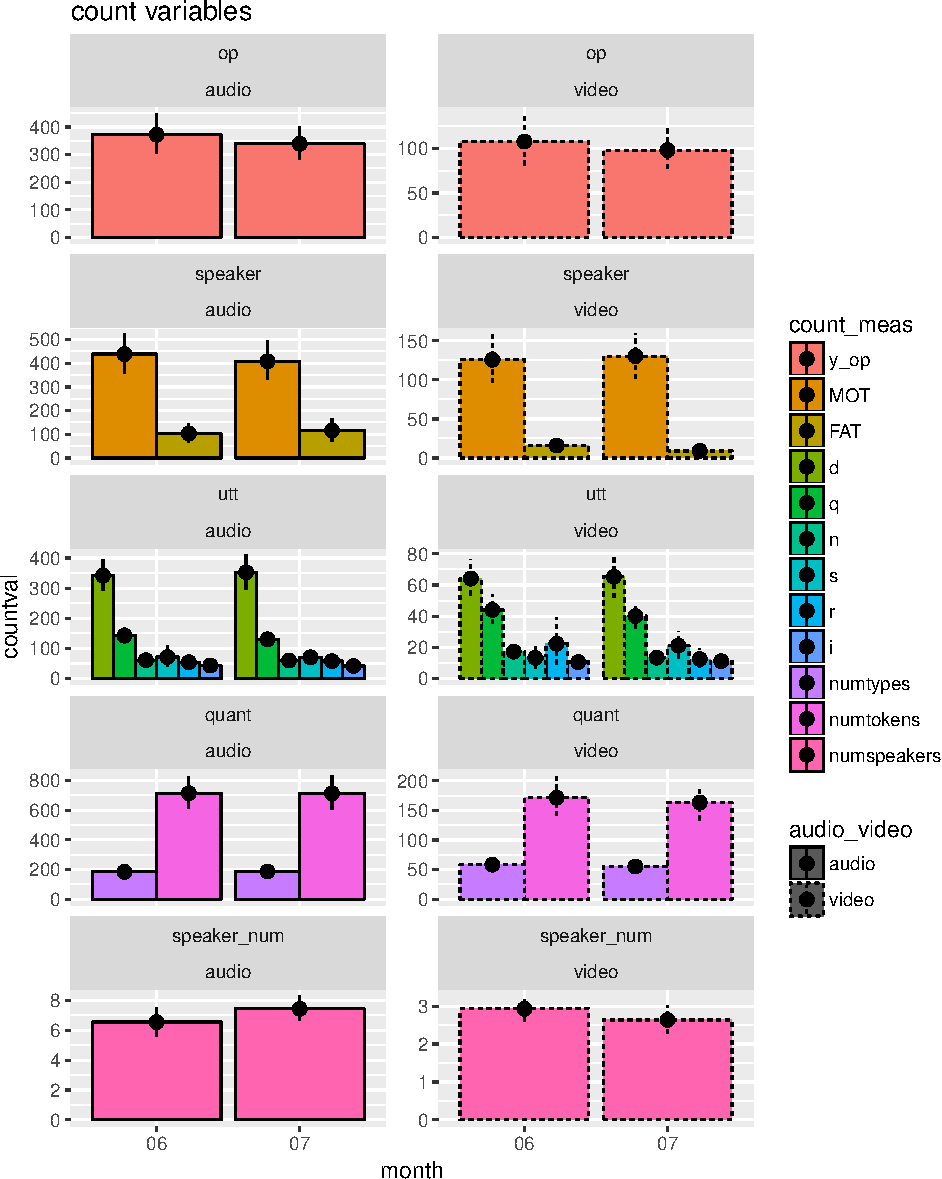
\includegraphics{sixseven_papaja_files/figure-latex/gr_derived_counts_67_diff-1.pdf}
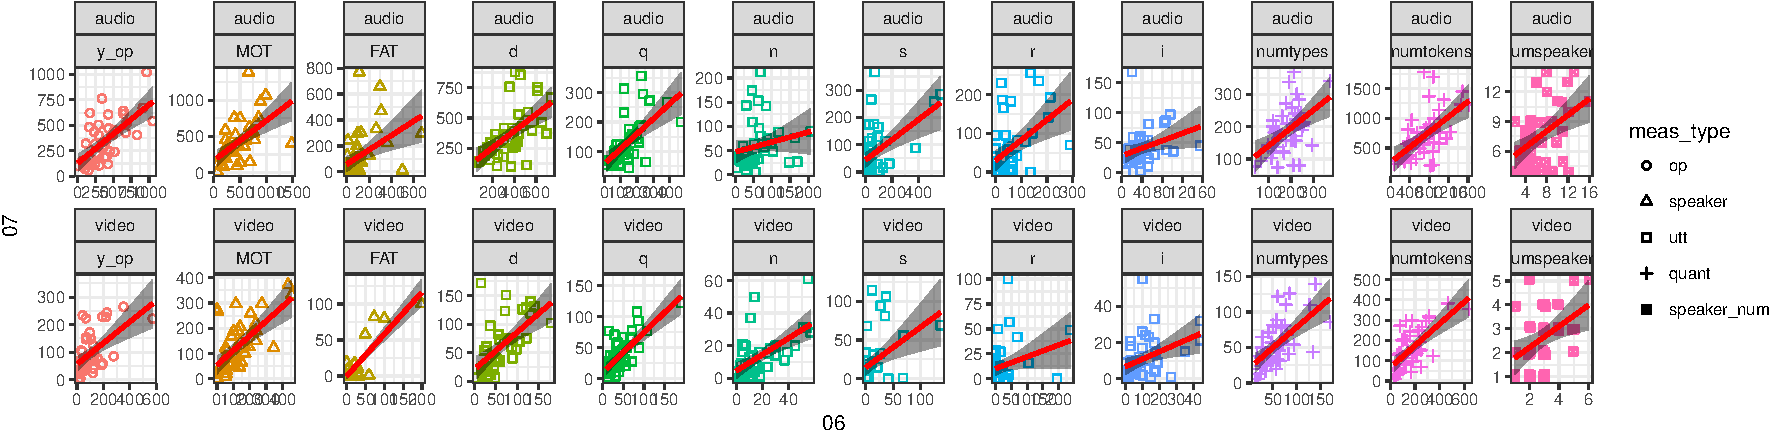
\includegraphics{sixseven_papaja_files/figure-latex/gr_derived_counts_67_corr-1.pdf}

\subsection{Count Measures, Audio-
vs.~Video-recordings}\label{count-measures-audio--vs.video-recordings}

We next assessed our count measures across recording-types, examing how
noun input scaled between hour-long video-recordings and daylong
audio-recordings. Modally, videos were an hour (62 min, \emph{M}=60.79,
SD=6.31, R=27.9-74.9 min), and audio-recordings were 16 hours (960 min,
\emph{M}=858.41, SD=119.41, R=635-960 min), the maximum capacity of the
LENA device. While determining the exact onsets and offsets of naps from
audio alone is not possible, by removing the \enquote{silent} portions
of the recordings (see Methods), we estimated an upper-limit on infants'
awake (i.e.~non-silent) time (Mode = 10.90, \emph{M} = 603, SD=106.8,
R=385.2-951 min ). This comports with established norms for
6--8-month-olds in the US (Mandel et al, 2010), which are 3 hours of
daytime sleep, and 10 hours of nighttime sleep. Thus, 16 hours of
recording beginning when the child wakes up should capture
\textasciitilde{}11 daytime waking hours, in line with our silence
demarcations. Infants were always awake during video recordings (save
one infant, who fell asleep before the recording-hour ended; that video
was stopped at sleep onset).

\begin{verbatim}
##   month aboost_min aboost_awakemin aboost_types aboost_tokens
## 1    06      13.89            9.88         4.05          5.79
## 2    07      14.82           10.45         4.65          6.03
##   aboost_speakers aboost_MOT aboost_FAT aboost_d aboost_q aboost_i
## 1            2.61       4.09       4.66     6.89     4.11     9.36
## 2            3.49       4.33      48.53     8.72     5.06    10.98
##   aboost_s aboost_r aboost_n aboost_op        comp
## 1     8.17     2.18     5.53      5.68 mean_aboost
## 2    10.31     8.64     8.44      6.07 mean_aboost
\end{verbatim}

\begin{verbatim}
##   month aboost_min aboost_awakemin aboost_types aboost_tokens
## 1    06       2.19            1.75         2.46          4.06
## 2    07       4.19            3.99         3.63          5.10
##   aboost_speakers aboost_MOT aboost_FAT aboost_d aboost_q aboost_i
## 1            1.74       3.13       3.77     4.77     3.15    12.52
## 2            2.13       3.74     139.61     8.76     5.60    27.00
##   aboost_s aboost_r aboost_n aboost_op      comp
## 1    10.20     2.11     4.88      5.55 sd_aboost
## 2    24.59    14.05    10.45      8.25 sd_aboost
\end{verbatim}

To examine how the hour-long video data \enquote{scale} to day-length
data descriptively, we divided the 12 audio count metrics by the 12
video count metrics for each child, to derive \enquote{audio-boost}
scores. This showed that the audio-recordings were \textasciitilde{}14x
longer than the videos, or 10x longer if only \enquote{non-silent}
portions of the audio-recording are included. However, rather than a
concomitant 10-fold increase in our count metrics (as would be expected
if the video captured a \enquote{representative} hour of the day), the
boost was closer to fivefold across measures; see Table XX. This
suggests that the videos, by and large, had a denser concentration of
nouns across our measures than did the audio recordings.

Notably, \enquote{zero} values (e.g.~recordings in which there were no
nouns heard in singing) were omitted from the audio-boost computations
given that they result in undefined values for a given child in a given
month. The majority of variables had at least one such value, with over
1/3 of video recordings lacking instances of nouns heard in singing,
reading, or by fathers each month; see Table XX.

\begin{verbatim}
## # A tibble: 2 x 11
##    month v_MOT a_FAT v_FAT   v_q   v_i   a_s   v_s   a_r   v_r   v_n
##   <fctr> <dbl> <dbl> <dbl> <dbl> <dbl> <dbl> <dbl> <dbl> <dbl> <dbl>
## 1     06  0.16  0.05  0.52  0.00  0.07  0.07  0.32  0.25  0.55  0.02
## 2     07  0.09  0.09  0.75  0.02  0.07  0.07  0.34  0.25  0.50  0.07
\end{verbatim}

\begin{verbatim}
## # A tibble: 1 x 8
##   v_MOT a_FAT v_FAT   v_i   a_s   v_s   a_r   v_r
##   <dbl> <dbl> <dbl> <dbl> <dbl> <dbl> <dbl> <dbl>
## 1  0.09  0.02  0.52  0.02  0.02  0.11  0.16  0.34
\end{verbatim}

We next normed our count values by the number of minutes in each. For
example, if an infant heard 500 noun-tokens in 800 minutes of non-silent
audio-recording, and 200 in 60 minutes of videos, this was normed to .62
and 3.3 noun-tokens per minute, respectively. Unlike for the audio-boost
calculation, this allows us to retain zero values, rendering more
readily interpretable results across our count and proportional
measures.

\begin{verbatim}
## # A tibble: 12 x 3
##      norm_meas  `06`  `07`
##         <fctr> <dbl> <dbl>
##  1        y_op   2.9   2.8
##  2         MOT   2.9   3.2
##  3         FAT   1.5   0.8
##  4           d   1.9   1.8
##  5           q   3.1   3.0
##  6           n   2.9   2.2
##  7           s   1.8   3.0
##  8           r   4.0   2.1
##  9           i   2.4   2.8
## 10    numtypes   3.1   2.9
## 11   numtokens   2.4   2.3
## 12 numspeakers   4.4   3.6
\end{verbatim}

With the normed data, we found identical patterns when looking within
month six and seven: /12 of our count-based metrics (in each month)
occurred at significantly lower rates in audio recordings than video
recordings (adjusted-p\textless{}.05). The three that were statistically
indistinguishable were nouns/minute produced (1) by fathers, (2) in
reading, and (3) in singing (all adjusted-p\textgreater{}.05). These
same three measures had a large number of zero values; see table XX. We
return to the topic of unattested low-frequency events in corpora in the
discussion.

The pattern of correlations across recording-types was mixed: in month
six, audio vs.~video normed count data only correlated significanly for
3/12 metrics, which were all utterance-type measures: declaratives (tau
= 0.44), questions (tau = 0.33), and imperatives (tau = 0.30; all 3
adjusted-p\textless{}.05). For month seven, 11/12 metrics correlated in
audio vs.~video data; number of nouns per minute heard in singing did
not (excluding singing, 0.27 - 0.53, all adjusted-p\textless{}.05). See
table XX and figure YY.

\begin{figure}[htbp]
\centering
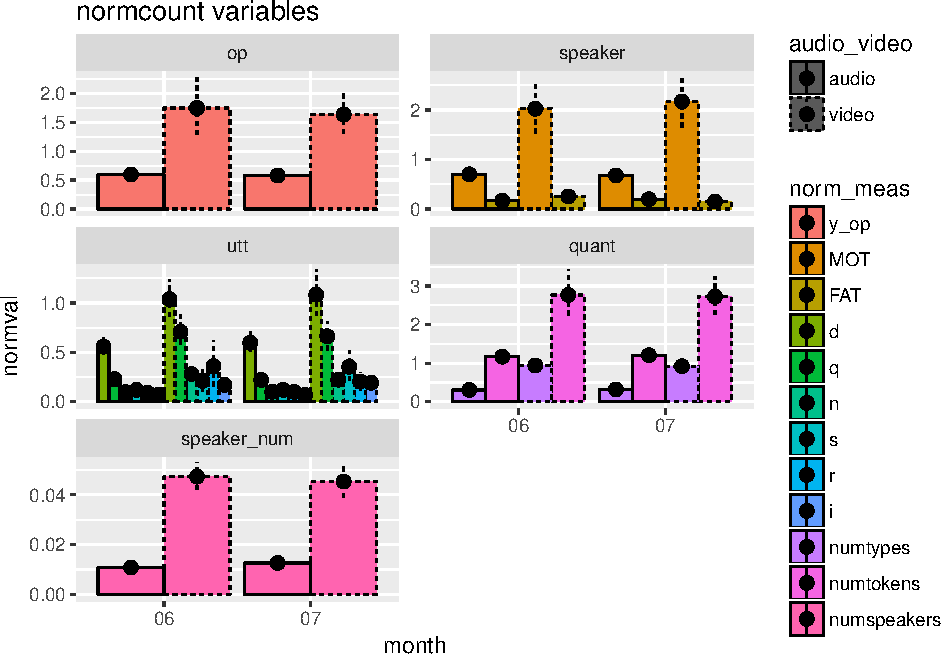
\includegraphics{sixseven_papaja_files/figure-latex/gr_derived_counts_diff-1.pdf}
\caption{}
\end{figure}

\begin{figure}[htbp]
\centering
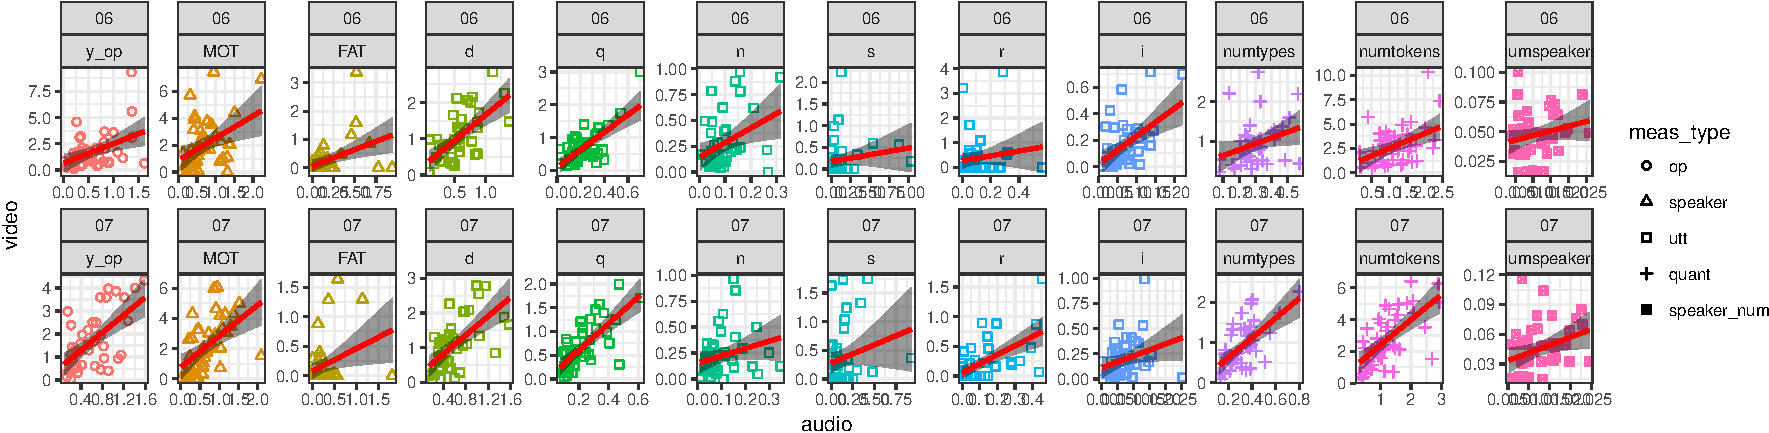
\includegraphics{sixseven_papaja_files/figure-latex/gr_derived_counts_corr-1.pdf}
\caption{}
\end{figure}

\subsection{Proportion Measures, Month 6
vs.~7.}\label{proportion-measures-month-6-vs.7.}

Turning to the 10 proportion measures, as with the count measures, there
were no significant differences between month six and seven within
audio- or within video-recordings (all adjusted-p\textgreater{}.05). The
pattern of correlations differed somewhat from the count measures: for
the audio-recordings, 7/10 proportional measures correlated from month 6
to 7 (for these seven: Kendall's tau range: 0.31-0.46,
adjusted-p\textless{}.05; for object co-presence, questions, and
short-phrases adjusted-p\textgreater{}.05). For videos, only proportion
of input from mom and from dad correlated significantly from month 6 to
7 (Kendall's tau = 0.45 and 0.63, respectively;
adjusted-p\textless{}.05). Thus, overall, the proportional metrics were
indistinguishable month-to-month within recording-type, but the
correlations between the proportional measures across children at month
six and seven were variable, especially for video-recordings.

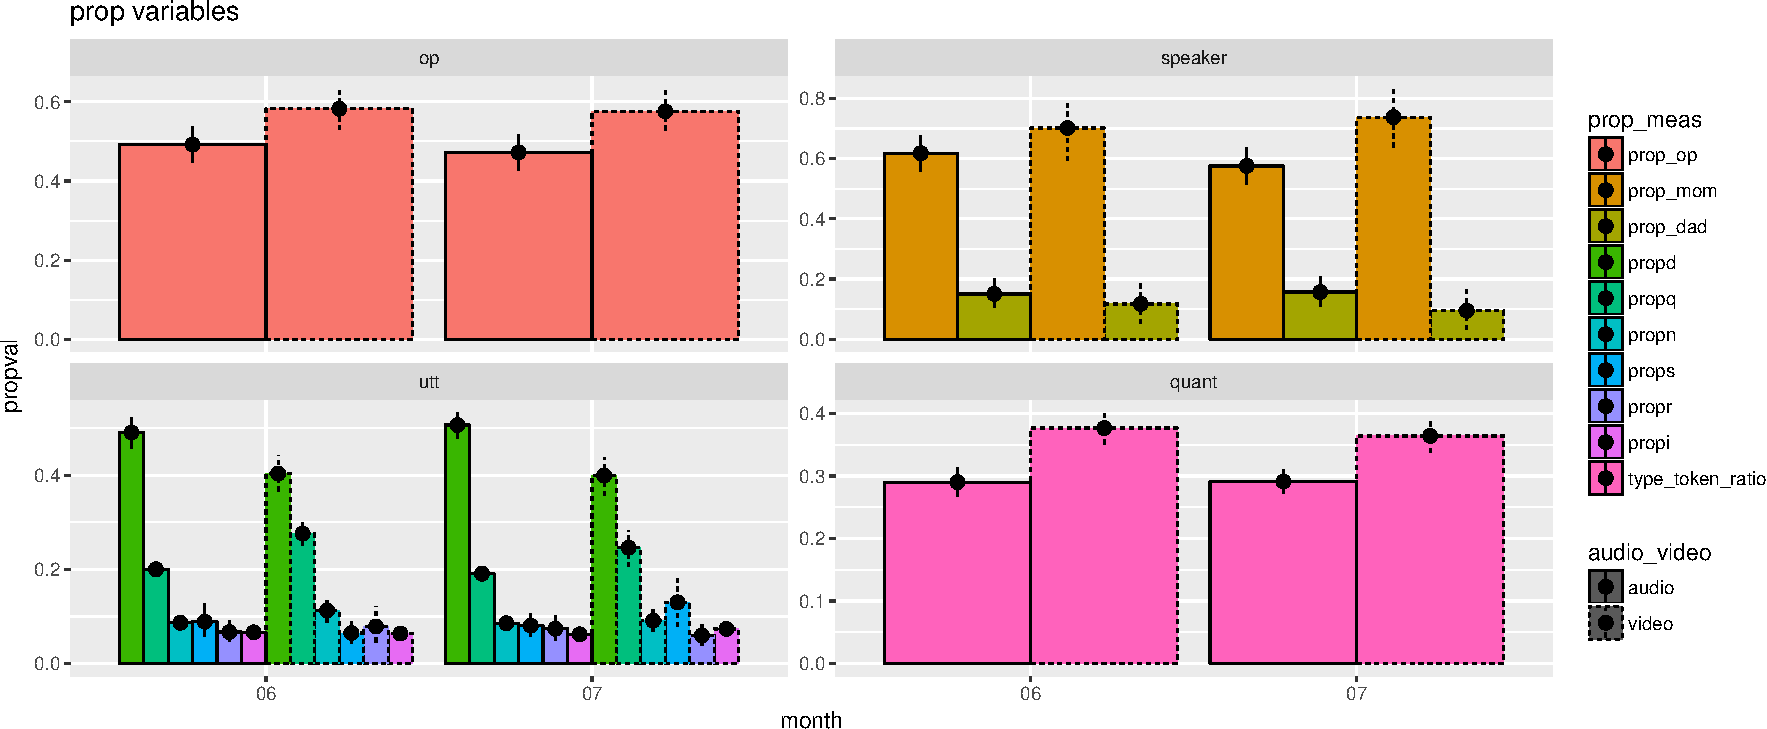
\includegraphics{sixseven_papaja_files/figure-latex/gr_derived_props-1.pdf}
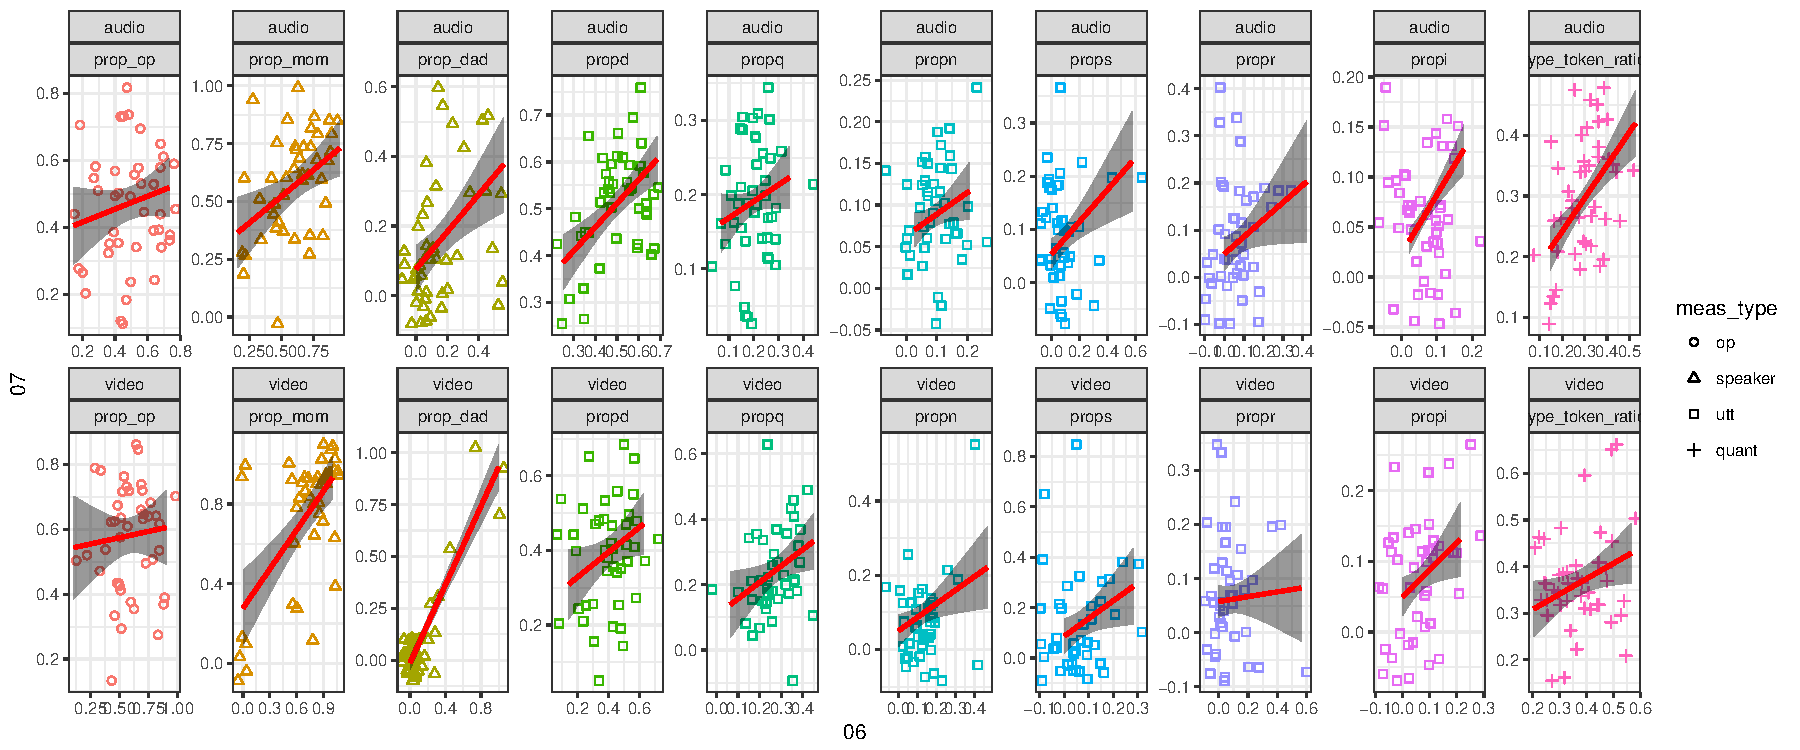
\includegraphics{sixseven_papaja_files/figure-latex/gr_derived_props-2.pdf}

\subsection{Proportion Measures, Audio-
vs.~Video-recordings}\label{proportion-measures-audio--vs.video-recordings}

Across recording-types, proportional measures differed more
substantively than count measures; see figure XX. At six months, 4/10
proportional measures differed significantly between audio- and
video-recordings (type-token ratio, and the proportion of object
presence, declaratives, and questions, all adj-p\textless{}.05), while
at seven months, 6/10 did so (the same four as in month six, plus input
from mothers and fathers; all adj-p\textless{}.05). See Figure XX.

Descriptively, videos featured object presence more than
audio-recordings (\(M_{\Delta}\) = \%), likely reflecting a narrower
range of activities during video recording. Videos also had a higher
type-to-token ratios (i.e.~more lexical diversity): \emph{M}= vs. for
audio-recordings, consistant with previous work (Covington \& Fall,
2010).

Across utterance-types, the overall distributions of nouns in audio- and
video-recordings were similar: the majority of the noun input was
declaratives, followed by questions, with the remaining input spread
across imperatives, reading, singing, and short-phrases; see Figure XX.
However, audio-recordings featured relatively more declaratives and
fewer questions than videos (, and \%, respectively). Finally, in month
seven, mothers talked \% less in audio than video, and fathers talked \%
more.

\begin{figure}[htbp]
\centering
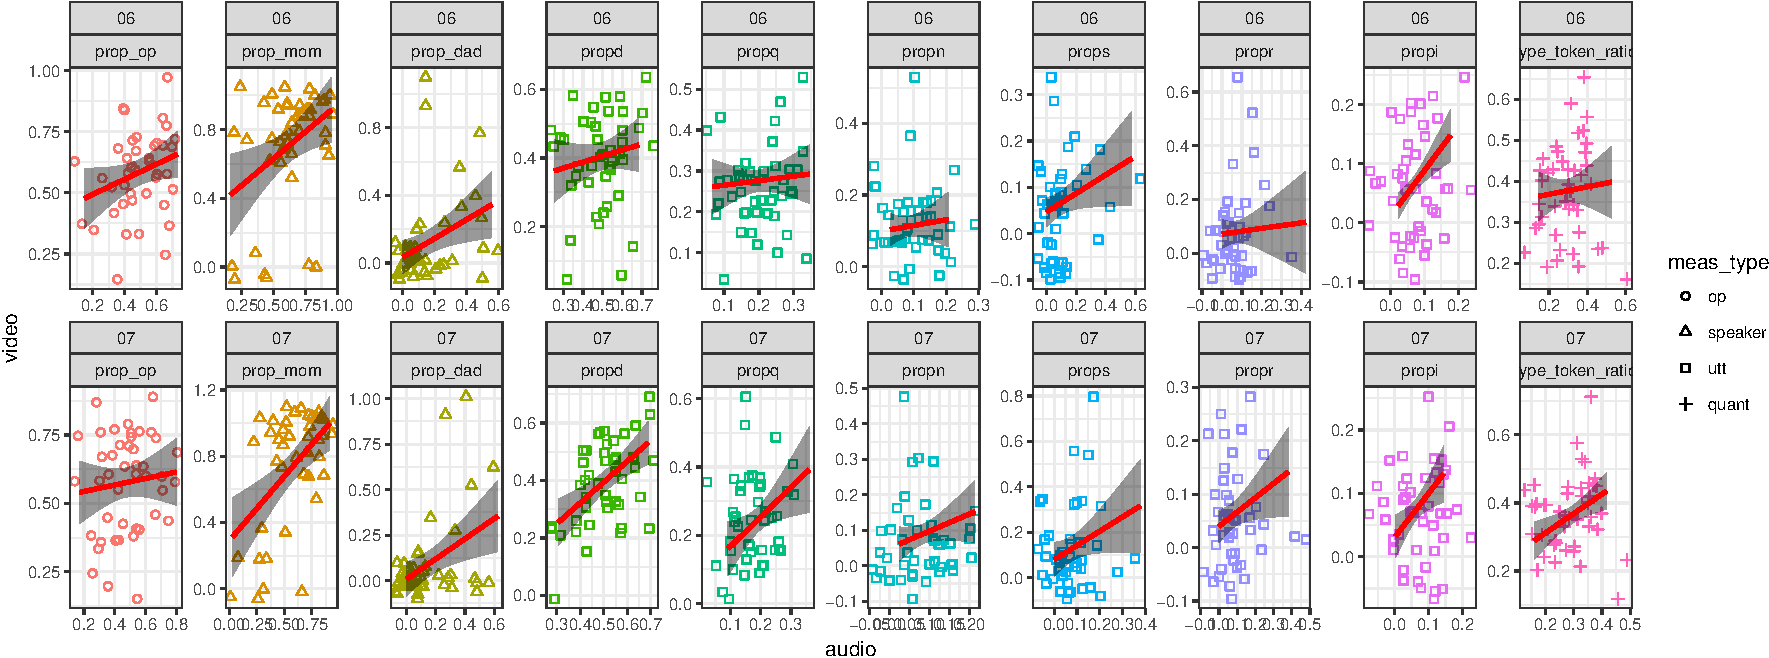
\includegraphics{sixseven_papaja_files/figure-latex/gr_derived_props_av-1.pdf}
\caption{}
\end{figure}

Turning to correlations across recording-types, in month six only the
proportion of imperatives reached significance (Kendall's tau =,
adj-p\textless{}.05). At seven months, three of the variables that
differed significantly also correlated significantly (proportion of noun
input from fathers and mothers, and in declaratives), along with the
proportion of nouns heard in reading, (all four adj-p\textless{}.05,
Kendall's tau range: 0.30 - 0.35).

\section{Noun Frequency and
Prevalence}\label{noun-frequency-and-prevalence}

We conclude with a set of highly exploratory analyses at the word level,
which aim to provide a first-pass characterization of whether audio and
video recordings captured the same nouns and the same relative
frequencies by examining word frequency across each month, recording
type, and infant. The distribution of nouns in our recordings was
zipfian: of the 5801unique object words (3137 lemmas) heard across
months and recording types, only 2482 (960 lemmas) were heard more than
once (see figure XX).

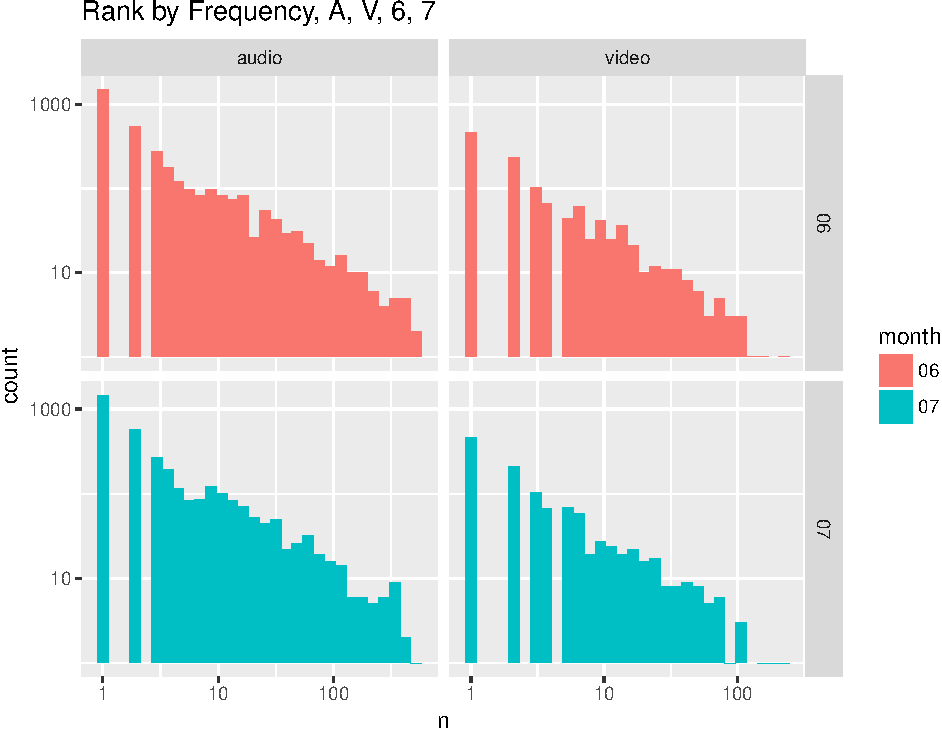
\includegraphics{sixseven_papaja_files/figure-latex/noun_freq-1.pdf}
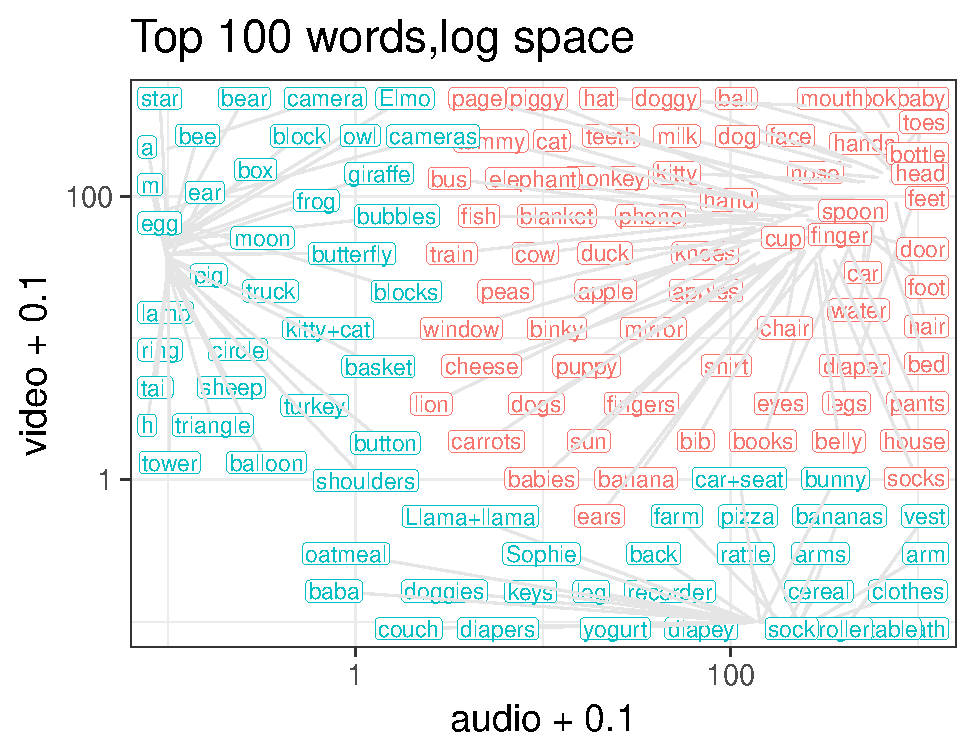
\includegraphics{sixseven_papaja_files/figure-latex/noun_freq-2.pdf}

Collapsing month, we examined the top 100 most frequent nouns from
audio- and video-recordings (n=136 due to ties, n=68 without words that
occurred zero times in one recording-type). Frequency across
recording-types correlated significantly (Kendall's tau: 0.39,
p\textless{}.0001,) even with zero-frequency words included (Kendall's
tau: 0.25, p\textless{}.0001; see figure XX). Further, we found
numerically stronger correlations month-to-month than across
recording-types within month (month 6 audio vs.~video: tau = 0.15, month
7 audio vs.~video: tau = 0.15, month 6 vs.~7 audio: tau = 0.50, month 6
vs.~7 video: tau = 0.26, all adjusted-p\textless{}.05; see figure XX).
Thus, at the word-level too, month-to-month measures appear more stable
than cross-recording-type measures

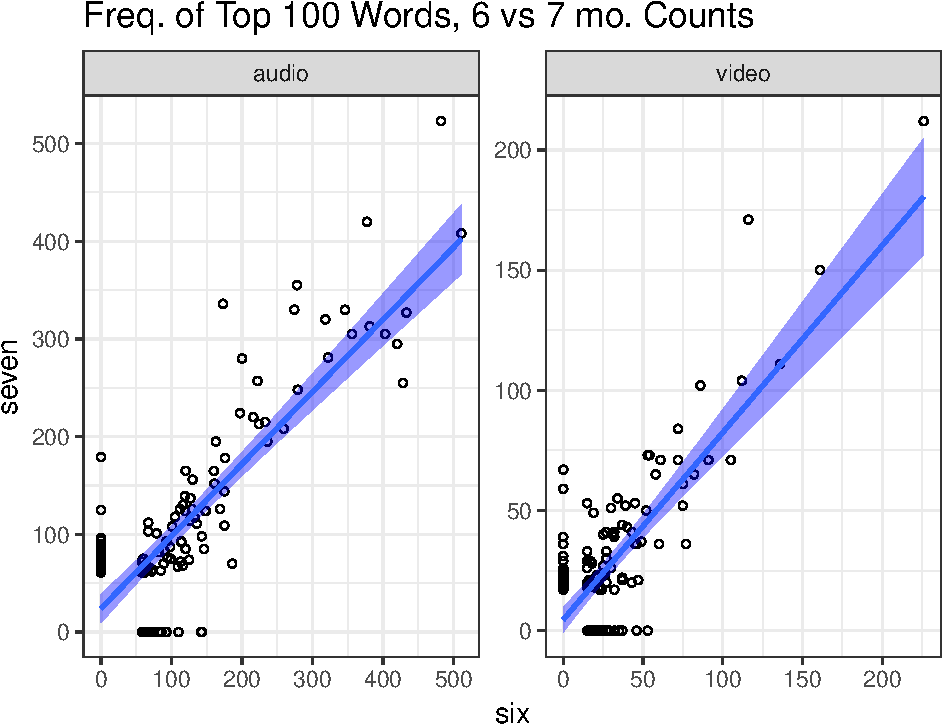
\includegraphics{sixseven_papaja_files/figure-latex/top100_corgraphs-1.pdf}
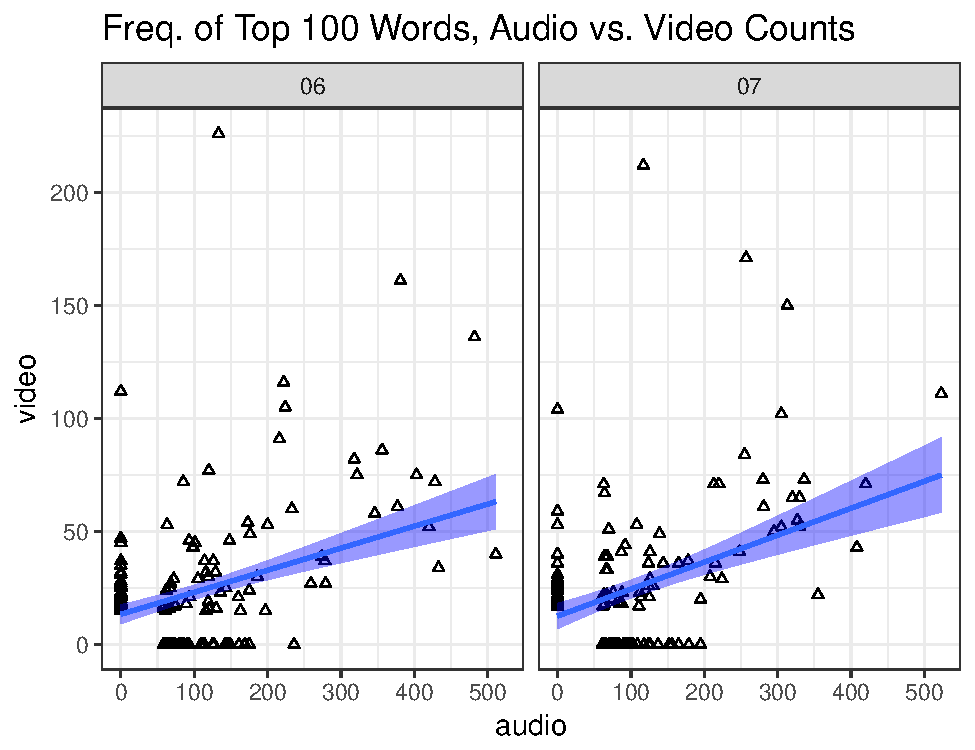
\includegraphics{sixseven_papaja_files/figure-latex/top100_corgraphs-2.pdf}

Finally, looking at just the top ten words by month and recording-type,
we again find greater consistency across months than recording-types
(see Figure XX and Table XX). Indeed, top words within recording-type
were largely overlapping, while only two words overlapped on all four
lists (book and baby). Furthermore, characterizing how words were spread
across infants and months, we find that the top audio words were far
more common across families than the top video words were (see figure
XX). Thus, daylong audio-recordings appear to render more stable
high-frequency words across families and across months than do
video-recordings.

\begin{figure}[htbp]
\centering
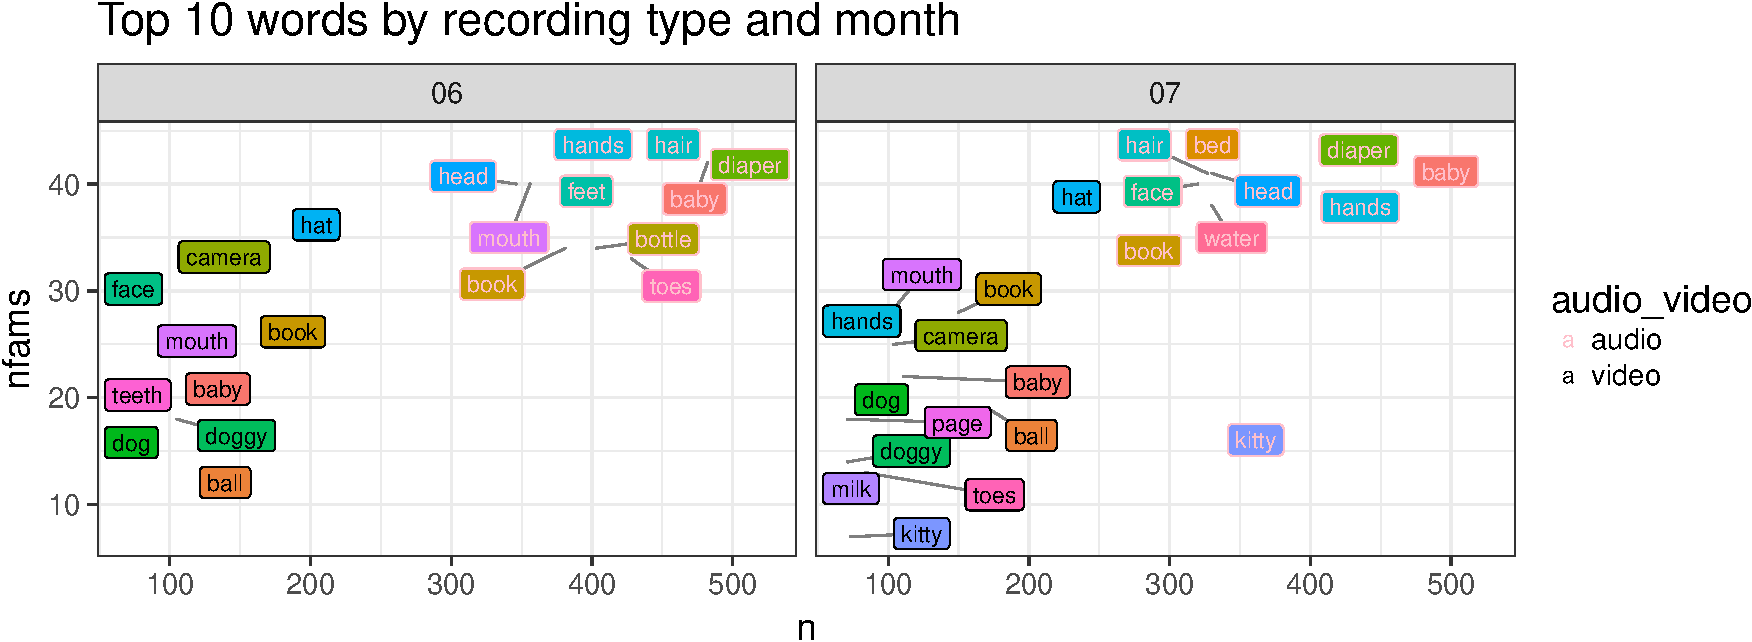
\includegraphics{sixseven_papaja_files/figure-latex/top10noun_freq-1.pdf}
\caption{}
\end{figure}

\section{Discussion}\label{discussion}

\newpage

\section{References}\label{references}

\setlength{\parindent}{-0.5in} \setlength{\leftskip}{0.5in}






\end{document}
